% Preamble
\documentclass[11pt,reqno,oneside,a4paper]{article}
\usepackage[a4paper,includeheadfoot,left=20mm,right=20mm,top=20mm,bottom=20mm]{geometry} %sets up the margins

%%%%%%%%%%%%%%%%%%%%%%%%%%%%%%%%%%%%%%%%%%%%%%%%%%%%%%%%%%%%%%%%%%%%%%%%%%%%%%%%
%
% This file contains some standard modifications to basic LaTeX2e and
% the article documentclass. Look through
% and make use of the shorthands defined herein.
%
%%%%%%%%%%%%%%%%%%%%%%%%%%%%%%%%%%%%%%%%%%%%%%%%%%%%%%%%%%%%%%%%%%%%%%%%%%%%%%%%

% Standard packages
\usepackage{amssymb,amsmath,amsthm}
\usepackage{xcolor,graphicx}
\usepackage{verbatim}
\usepackage{hyperref}
% Layout of headers & footers
\usepackage{titling}
\usepackage{fancyhdr}
\pagestyle{fancy} \lhead{{\theauthor}} \chead{} \rhead{} \lfoot{} \cfoot{\thepage} \rfoot{}

% Hyphenation
\hyphenation{non-zero}

% Instructor's email address
\newcommand{\InstEmail}{dave.smith@yale-nus.edu.sg}

%% Mathmode shortcuts
% Number sets
\newcommand{\NN}{\mathbb N}              % The set of naturals
\newcommand{\NNzero}{\NN^0}              % The set of naturals including zero
\newcommand{\NNone}{\NN}                 % The set of naturals excluding zero
\newcommand{\ZZ}{\mathbb Z}              % The set of integers
\newcommand{\QQ}{\mathbb Q}              % The set of rationals
\newcommand{\RR}{\mathbb R}              % The set of reals
\newcommand{\CC}{\mathbb C}              % The set of complex numbers
\newcommand{\KK}{\mathbb K}              % An arbitrary field
% Modern typesetting for the real and imaginary parts of a complex number
\renewcommand{\Re}{\operatorname*{Re}} \renewcommand{\Im}{\operatorname*{Im}}
% Upright d for derivatives
\newcommand{\D}{\ensuremath{\,\mathrm{d}}}
% Make epsilons look more different from the element symbol
\renewcommand{\epsilon}{\varepsilon}
% Always use slanted forms of \leq, \geq
\renewcommand{\geq}{\geqslant}
\renewcommand{\leq}{\leqslant}
% Shorthand for some relations
\newcommand{\po}{\preceq}
\newcommand{\rel}{{\mathcal R}} \newcommand{\rels}{\mathbin{\scriptstyle{\mathcal R}}}
% Shorthand for "if and only if" symbol
\newcommand{\Iff}{\ensuremath{\Leftrightarrow}}
% Make bold symbols for vectors
\providecommand{\BVec}[1]{\mathbf{#1}}
% Barred forms of \oplus and \otimes to represent the descents of these binary operators
\newcommand{\oplusbar}{\mathbin{\ooalign{$\hidewidth\overline{\oplus}\hidewidth$\cr$\phantom{\oplus}$}}} \newcommand{\otimesbar}{\mathbin{\ooalign{$\hidewidth\overline{\otimes}\hidewidth$\cr$\phantom{\otimes}$}}}
% Mathematical operators used in Proof
\DeclareMathOperator{\sgn}{sgn}          % The signum of a real number
\DeclareMathOperator{\power}{\mathcal{P}} % The power set of a set
\DeclareMathOperator{\Id}{Id}            % The identity function
\DeclareMathOperator{\Fun}{Fun}          % The set of functions from one set to another
\DeclareMathOperator{\Perm}{Perm}        % The set of permutations on a set
\DeclareMathOperator{\GCD}{GCD}          % The greatest common divisor of two integers
\newcommand{\abs}[1]{\left\lvert#1\right\rvert} % The absolute value of a real number or modulus of a complex number, with automatically scaling delimiters


%%%%%%%%%%
% Define extra macros here, if you need them.
%%%%%%%%%%






% Theorem definitions in the amsthm standard
\newtheorem{thm}{Theorem}
\newtheorem{lem}[thm]{Lemma}
\newtheorem{sublem}[thm]{Sublemma}
\newtheorem{prop}[thm]{Proposition}
\newtheorem{cor}[thm]{Corollary}
\newtheorem{conc}[thm]{Conclusion}
\newtheorem{conj}[thm]{Conjecture}
\theoremstyle{definition}
\newtheorem{defn}[thm]{Definition}
\newtheorem{cond}[thm]{Condition}
\newtheorem{asm}[thm]{Assumption}
\newtheorem{ntn}[thm]{Notation}
\newtheorem{prob}[thm]{Problem}
\theoremstyle{remark}
\newtheorem{rmk}[thm]{Remark}
\newtheorem{eg}[thm]{Example}
\newtheorem*{hint}{Hint}

% \usepackage{tikz}

\title{Final problem}
\author{NAMES}

% Document
\begin{document} %\pagenumbering{gobble}

\maketitle
\thispagestyle{fancy}

This document will contain the solution to the final problem of the module.

\tableofcontents

\clearpage
\section{Problem} \label{sec:Problem}
The statement of the problem.


\clearpage
\section{Preliminaries} \label{sec:Preliminaries}
%preliminaries
Let $\hat{\phi}$ represent the spatial Fourier Transform, i.e.
$$\widehat{\phi}(\lambda) := \int_{-\infty}^{\infty} \phi(x) e^{-i\lambda x} \mathrm{d}x = \int_{0}^{1} \phi(x) e^{-i\lambda x} \mathrm{d}x.$$
Then, using integration by parts,
\begin{align*}
    \widehat{\frac{\mathrm{d}^3}{\mathrm{d}x^3}\phi}(\lambda) &= \int_{0}^{1} \phi'''(x) e^{-i\lambda x} \mathrm{d}x \\
    &= \phi''(x) e^{-i\lambda x}\bigg\rvert_0^1 + i\lambda\int_{0}^{1} \phi''(x) e^{-i\lambda x} \mathrm{d}x \\
    &= \left(\phi''(x) e^{-i\lambda x} + i\lambda \phi'(x) e^{-i\lambda x} \right)\bigg\rvert_0^1 - \lambda^2\int_{0}^{1} \phi'(x) e^{-i\lambda x} \mathrm{d}x \\
    &= \left(\phi''(x) e^{-i\lambda x} + i\lambda \phi'(x) e^{-i\lambda x} - \lambda^2 \phi(x) e^{-i\lambda x}\right) \bigg\rvert_0^1 - i\lambda^3\int_{0}^{1} \phi(x) e^{-i\lambda x} \mathrm{d}x \\
    &= \left(\phi''(x) e^{-i\lambda x} + i\lambda \phi'(x) e^{-i\lambda x} - \lambda^2 \phi(x) e^{-i\lambda x}\right) \bigg\rvert_0^1 - i\lambda^3\widehat\phi(\lambda). \\
\end{align*}

\clearpage
\section{Stage 1} \label{sec:Stage1}
%stage 1
We were given the PDE
$$[\partial_t+\partial_{xxx}]q(x,t) = 0.$$
Perform a spatial Fourier Transform of the PDE, using our Preliminary Work, we get
\begin{align*}
    \widehat{[\partial_t+\partial_{xxx}]q}(x,t) &= \widehat{\partial_t q}(\lambda,t) + e^{-i\lambda x}\left(\partial_{xx}q(x,t) + i\lambda \partial_{x}q(x,t) - \lambda^2 q(x,t) \right) \bigg\rvert_0^1 - i \lambda^3\widehat{q}(\lambda,t) \\
    &= (\partial_t - i \lambda^3) \widehat{q}(\lambda,t) + e^{-i\lambda x}\left(\partial_{xx}q(x,t) + i\lambda \partial_{x}q(x,t) - \lambda^2 q(x,t) \right) \bigg\rvert_0^1 \\
    &= 0.
\end{align*}
Therefore, we have the ODE
\begin{align*}
&[\partial_t - i \lambda^3] \widehat{q}(\lambda,t) + e^{-i\lambda}\left(\partial_{xx}q(1,t) + i\lambda \partial_{x}q(1,t) - \lambda^2 q(1,t)\right) - \partial_{xx}q(0,t) - i\lambda \partial_{x}q(0,t) + \lambda^2 q(0,t) \\
&= 0.
\end{align*}
Multiply both sides by $e^{-i\lambda^3 t}$ to get
\begin{align*}
&e^{-i\lambda^3 t}[\partial_t - i \lambda^3] \widehat{q}(\lambda,t) + e^{-i\lambda -i\lambda^3 t}\left(\partial_{xx}q(1,t) + i\lambda \partial_{x}q(1,t) - \lambda^2 q(1,t)\right) \\
&- e^{-i\lambda^3 t}\left(\partial_{xx}q(0,t) + i\lambda \partial_{x}q(0,t) - \lambda^2 q(0,t)\right) \\
&= 0.
\end{align*}
Observe that
    $$e^{-i\lambda^3 t}[\partial_t - i \lambda^3] \widehat{q}(\lambda,t) = \frac{\mathrm{d}}{\mathrm{d}t}\left(e^{-i\lambda^3 t}\widehat{q}(\lambda,t)\right).$$
Integrate with respect to time to solve the ODE,
\begin{align*}
&\int_0^t \frac{\mathrm{d}}{\mathrm{d}s} \left(e^{-i\lambda^3 s} \widehat{q}(\lambda,s)\right) \mathrm{d}s \\
&-\int_0^t e^{-i\lambda^3 s}\left(\partial_{xx}q(0,s) + i\lambda \partial_{x}q(0,s) - \lambda^2 q(0,s)\right) \mathrm{d}s \\
&+\int_0^t e^{-i\lambda -i\lambda^3 s}\left(\partial_{xx}q(1,s) + i\lambda \partial_{x}q(1,s) - \lambda^2 q(1,s)\right) \mathrm{d}s \\
&= 0.
\end{align*}

We will introduce the notation
$$f_j(\lambda,X,t) := \int_0^t e^{-i\lambda^3 s}(\partial_x)^j q(X,s) \mathrm{d}s.$$
Therefore, we get
\begin{align*}
&e^{-i\lambda^3 t} \widehat{q}(\lambda,t) - \widehat{q}(\lambda,0) \\
&-\left(f_2(\lambda,0,t) + i\lambda f_1(\lambda,0,t) - \lambda^2 f_0(\lambda,0,t)\right) \\
&+e^{-i\lambda}\left(f_2(\lambda,1,t) + i\lambda f_1(\lambda,1,t) - \lambda^2 f_0(\lambda,1,t)\right) \\
&= 0
\end{align*}
which implies that
\begin{align*}
\widehat{q}(\lambda,t) = e^{i\lambda^3 t} \widehat{q}(\lambda,0) &+e^{i\lambda^3 t}\left(f_2(\lambda,0,t) + i\lambda f_1(\lambda,0,t) - \lambda^2 f_0(\lambda,0,t)\right) \\
&-e^{-i\lambda+i\lambda^3 t}\left(f_2(\lambda,1,t) + i\lambda f_1(\lambda,1,t) - \lambda^2 f_0(\lambda,1,t)\right)
\end{align*}
and this equation is the Global Relation (GR) which is valid for all $\lambda \in \mathbb{C}$ and for all $t \in [0,T]$. Take the inverse spatial Fourier Transform of GR and split the integrals on the left-hand side to get equation 6
\begin{align}
2\pi q(x,t) &= \int_{-\infty}^{\infty} e^{i\lambda x + i\lambda^3 t} \widehat{q}_0(\lambda) \mathrm{d}\lambda \label{eqn:IFT_GR}\\ 
&+ \int_{-\infty}^{\infty} e^{i\lambda (x-1)+i\lambda^3 t}\left(f_2(\lambda,1,t) + i\lambda f_1(\lambda,1,t) - \lambda^2 f_0(\lambda,1,t)\right) \mathrm{d}\lambda \nonumber \\
&- \int_{-\infty}^{\infty} e^{i\lambda x+i\lambda^3 t}\left(f_2(\lambda,0,t) + i\lambda f_1(\lambda,0,t) - \lambda^2 f_0(\lambda,0,t)\right) \mathrm{d}\lambda. \nonumber
\end{align}

We aim to deform the latter two contours of integration away from $\mathbb{R}$. Define
\begin{align*}
    &\mathbb{C}^{\pm} := \{\lambda \in \mathbb{C} \mid \mbox{Im}(\lambda) > 0 \} \\
    &D := \{ \lambda \in \mathbb{C} \mid \mbox{Re}(-i\lambda^3) < 0 \} &D^{\pm} := D \cap \mathbb{C}^{\pm} \\
    &E := \{ \lambda \in \mathbb{C} \mid \mbox{Re}(-i\lambda^3) > 0 \} &E^{\pm} := E \cap \mathbb{C}^{\pm}
\end{align*}
and orient the boundaries of these (unions of) sectors in the positive sense; the sector lies to the left of its boundary.
Note that if we let $\lambda = e^{i\theta}$ for some $\theta \in \mathbb{R}$, then we can re-write sets $D$ and $E$ as
\begin{align*}
    &D = \{ e^{i\theta} \in \mathbb{C} \mid \cos(3\theta - \frac{\pi}{2}) < 0 \} \\
    &E = \{ e^{i\theta} \in \mathbb{C} \mid \cos(3\theta - \frac{\pi}{2}) > 0 \}. \\
\end{align*}
Refer to figure \ref{fig:intcontour} for a diagram of the sectors $D^{\pm}$ and $E^{\pm}$ on the complex plane.
\begin{figure}
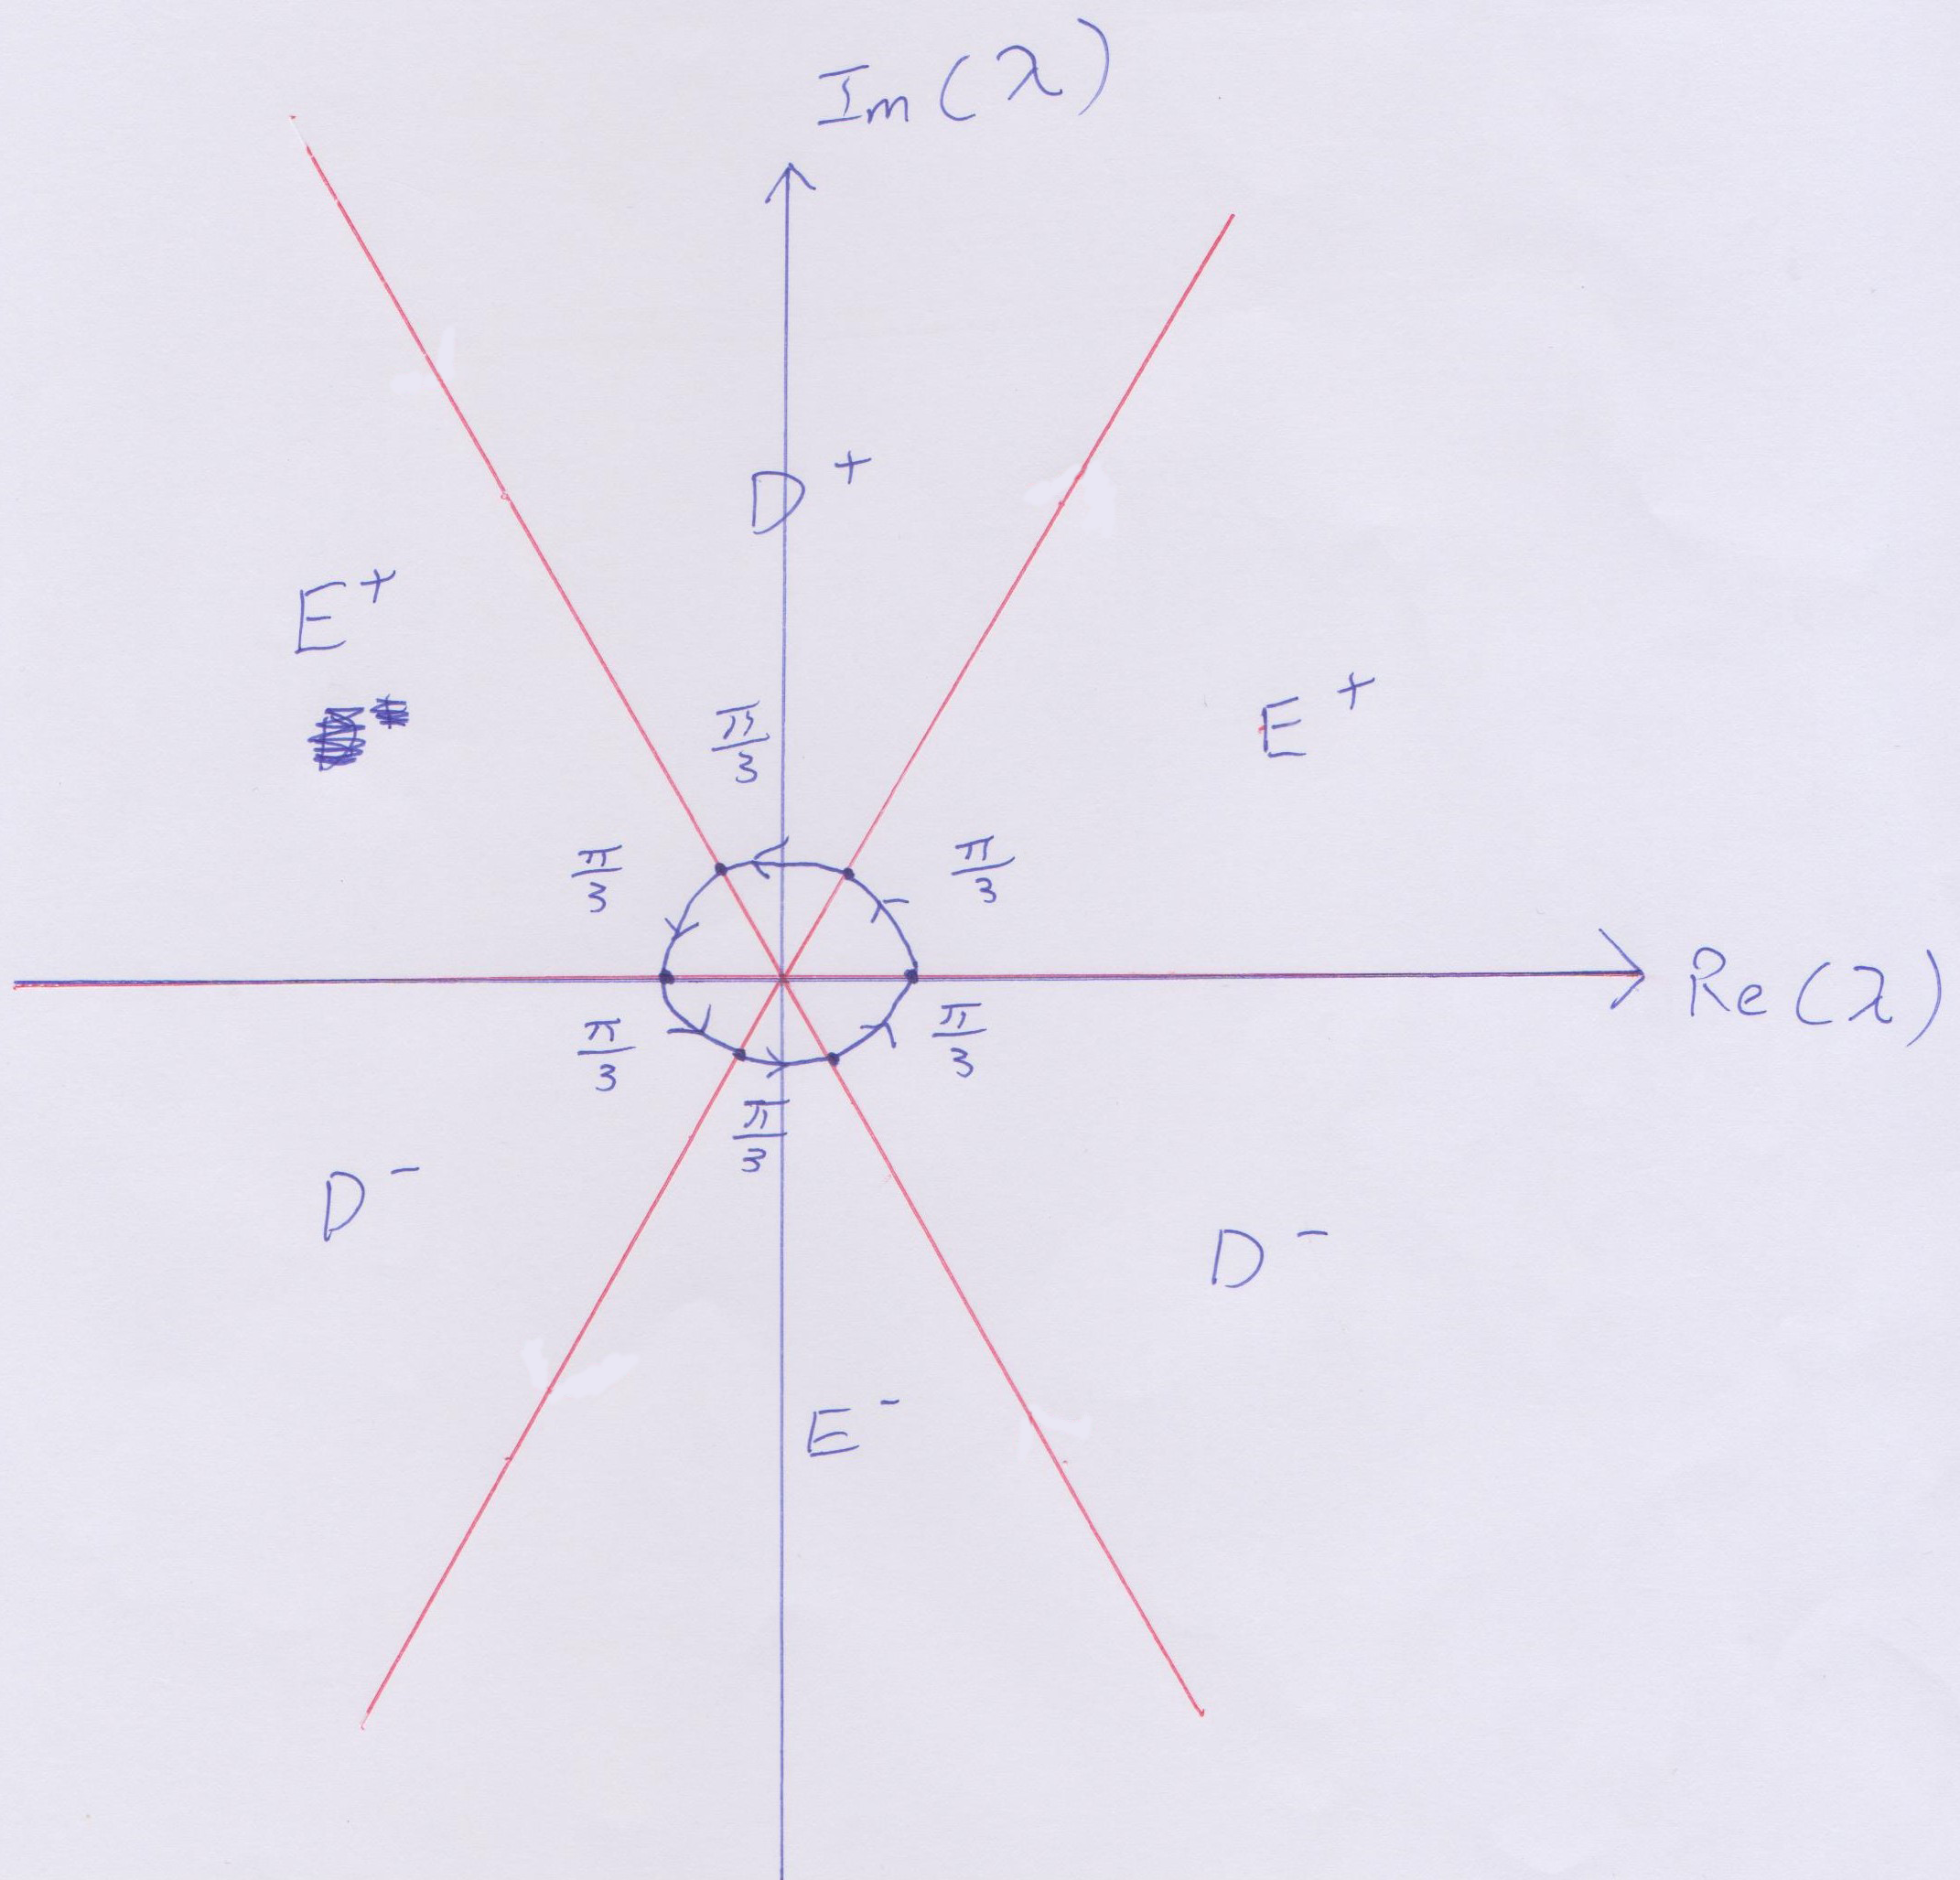
\includegraphics[width=\linewidth]{ImagesforFinalProblem/intcontour1.png}
\caption{A diagram showing the sectors $D^{\pm}$ and $E^{\pm}$ on the complex plane.}
\centering\label{fig:intcontour}
\end{figure}
\newpage Consider
$$f_j(\lambda,X,t) := \int_0^t e^{-i\lambda^3 s}(\partial_x)^j q(X,s) \mathrm{d}s,$$
multiply both sides by $e^{i\lambda^3 t}$ and integrate by parts in $s$, then
\begin{align*}
    e^{i\lambda^3 t}f_j(\lambda,X,t) &= \int_0^t e^{i\lambda^3 (t-s)}(\partial_x)^j q(X,s) \mathrm{d}s \\
    &= \frac{i}{i\lambda^3} e^{i\lambda^3 (t-s)}(\partial_x)^j q(X,s) \bigg\rvert_{s=0}^{s=t} - \frac{i}{\lambda^3}\int_0^t e^{i\lambda^3 (t-s)}(\partial_x)^j q(X,s) \mathrm{d}s. 
\end{align*}
$E$ was chosen so that Re($i\lambda^3(t-s)) \leq 0$ for all $s \in [0,t]$. Therefore, as $\lambda \rightarrow \infty$ within clos$(E)$, $e^{i\lambda^3 (t-s)} = \mathcal{O}(1)$ decays uniformly in arg$(\lambda)$, and by the Riemann-Lebesgue lemma, the integral in the second term is oscillatory. Therefore, $e^{i\lambda^3 t}f_j(\lambda,X,t)$ decays uniformly in arg$(\lambda)$ with $\mathcal{O}(\abs{\lambda^{-3}})$, which implies that the entire term
$$e^{i\lambda^3 t}\left(f_2(\lambda,0,t) + i\lambda f_1(\lambda,0,t) - \lambda^2 f_0(\lambda,0,t)\right) = \mathcal{O}(\abs{\lambda^{-1}}),$$
decays uniformly in arg$(\lambda)$ as $\lambda \rightarrow \infty$ within clos$(E)$.
Also, 
$$e^{i\lambda^3 t}\left(f_2(\lambda,0,t) + i\lambda f_1(\lambda,0,t) - \lambda^2 f_0(\lambda,0,t)\right) = \mathcal{O}(\abs{\lambda^{-1}})$$
is entire, i.e. analytic at all finite points of $\mathbb{C}$, as $(\partial_x)^jq(X,\cdot) \in L^1[0, T]$. Hence, by Jordan's lemma,
$$
    \int_{E^+} e^{i\lambda x+i\lambda^3 t}\left(f_2(\lambda,0,t) + i\lambda f_1(\lambda,0,t) - \lambda^2 f_0(\lambda,0,t)\right) \mathrm{d}\lambda = 0,
$$ 
and similarly,
$$
    \int_{E^-} e^{i\lambda (x-1)+i\lambda^3 t}\left(f_2(\lambda,1,t) + i\lambda f_1(\lambda,1,t) - \lambda^2 f_0(\lambda,1,t)\right) \mathrm{d}\lambda = 0.
$$
Temporarily denote
\begin{align*}
    &I_2 := e^{i\lambda (x-1)+i\lambda^3 t}\left(f_2(\lambda,1,t) + i\lambda f_1(\lambda,1,t) - \lambda^2 f_0(\lambda,1,t)\right), \\
    &I_3 := e^{i\lambda x+i\lambda^3 t}\left(f_2(\lambda,0,t) + i\lambda f_1(\lambda,0,t) - \lambda^2 f_0(\lambda,0,t)\right), \\
\end{align*} then,
\begin{align*}
    &\int_{-\infty}^{\infty} I_2 \mathrm{d}\lambda = -\int_{\infty}^{-\infty} I_2 \mathrm{d}\lambda = -\left\{\int_{\infty}^{-\infty} - \int_{E^-}\right\} I_2 \mathrm{d}\lambda = -\int_{D^-} I_2 \mathrm{d}\lambda \\
    &\int_{-\infty}^{\infty} I_3 \mathrm{d}\lambda = \left\{\int_{-\infty}^{\infty} - \int_{E^+}\right\} I_3 \mathrm{d}\lambda = \int_{D^+} I_3 \mathrm{d}\lambda. \\
\end{align*}
Therefore, we can re-write equation \ref{eqn:IFT_GR} as
\begin{align}
2\pi q(x,t) &= \int_{-\infty}^{\infty} e^{i\lambda x + i\lambda^3 t} \widehat{q}_0(\lambda) \mathrm{d}\lambda \label{eqn:EFt}\\ 
&- \int_{D^-} e^{i\lambda (x-1)+i\lambda^3 t}\left(f_2(\lambda,1,t) + i\lambda f_1(\lambda,1,t) - \lambda^2 f_0(\lambda,1,t)\right) \mathrm{d}\lambda \nonumber \\
&- \int_{D^+} e^{i\lambda x+i\lambda^3 t}\left(f_2(\lambda,0,t) + i\lambda f_1(\lambda,0,t) - \lambda^2 f_0(\lambda,0,t)\right) \mathrm{d}\lambda \nonumber
\end{align}
and this is the Ehrenpresis form (EFt) which is valid for $(x,t) \in (0,1) \times [0,T].$

By a similar argument, $\forall \tau \in [t,T],$ Re($i\lambda^3(t-s)) \leq 0$ within clos$(D)$ and therefore,
$$\int_t^\tau e^{i\lambda^3 (t-s)}\left(\partial_{xx}q(0,s) + i\lambda \partial_{x}q(0,s) - \lambda^2 q(0,s)\right) \mathrm{d}s$$
decays uniformly in arg$(\lambda)$ as $\lambda \rightarrow \infty$ within clos$(D)$.
Therefore, by Jordan's lemma, for sufficiently large $t$,
$$
    \int_{D^+} e^{i\lambda x+i\lambda^3 t}\left(f_2(\lambda,0,t) + i\lambda f_1(\lambda,0,t) - \lambda^2 f_0(\lambda,0,t)\right) \mathrm{d}\lambda = 0
$$
and
$$
    \int_{D^-} e^{i\lambda (x-1)+i\lambda^3 t}\left(f_2(\lambda,1,t) + i\lambda f_1(\lambda,1,t) - \lambda^2 f_0(\lambda,1,t)\right) \mathrm{d}\lambda = 0.
$$
This allows us to further manipulate equation \ref{eqn:EFt} to
\begin{align}
2\pi q(x,t) &= \int_{-\infty}^{\infty} e^{i\lambda x + i\lambda^3 t} \widehat{q}_0(\lambda) \mathrm{d}\lambda \label{eqn:EFtfinal}\\ 
&- \int_{D^-} e^{i\lambda (x-1)+i\lambda^3 t}\left(f_2(\lambda,1,t) + i\lambda f_1(\lambda,1,t) - \lambda^2 f_0(\lambda,1,t)\right) \mathrm{d}\lambda \nonumber \\
&- \int_{D^+} e^{i\lambda x+i\lambda^3 t}\left(f_2(\lambda,0,t) + i\lambda f_1(\lambda,0,t) - \lambda^2 f_0(\lambda,0,t)\right) \mathrm{d}\lambda \nonumber
\end{align}
which is valid for $(x,t) \in (0,1) \times [0,\tau], \tau \in [0,T]$ (in practice we will pick $\tau$ to be larger than all the time-values we care about).
This formula (EF$\tau$) has the advantage of very simple $(x,t)$ dependence.

We started by assuming that a solution exists and showed that any solution must satisfy (EF$\tau$) and (GR). 
The importance of the equation (GR) is not yet clear, except for deriving (EF$\tau$). 
Moreover, (EF$\tau$) is not an explicit representation of the solution since
\begin{enumerate}
    \item $f_1(\lambda,0,t)$
    \item $f_2(\lambda,0,t)$
    \item $f_2(\lambda,1,t)$
\end{enumerate}
are unknown.

% \clearpage
% \section{} \label{sec:}
% \input{../final-problem/???}


\end{document}


